\documentclass[]{final_report}
\usepackage{graphicx}
\usepackage{hyperref}
\usepackage{titlesec}
\usepackage[utf8]{inputenc}
\usepackage[backend=biber, style=ieee]{biblatex}
\usepackage{amsmath}
\usepackage{amssymb}
\usepackage{float}
\usepackage{tabularx} % Needed for the X column type
\usepackage{booktabs} % For prettier tables
\usepackage{lipsum}   % For dummy text


\addbibresource{fyp.bib}
\usepackage{amsthm}
\theoremstyle{definition}
\newtheorem{definition}{Definition}[chapter]
\newtheorem{basic}{Basic Definition}

%%%%%%%%%%%%%%%%%%%%%%
%%% Input project details
\def\studentname{Jude Asare}
\def\reportyear{2023/2024}
\def\projecttitle{Implementing the PKCS\#1 v1.5 Signature Scheme with provably secure parameters}
\def\supervisorname{Saqib Kakvi}
\def\degree{MSci (Hons) in Computer Science (Information Security)}
\def\fullOrHalfUnit{Appendix A} 
\begin{document}


%%%%%%%%%%%%%%%%%%%%%%
%%% Table of Contents
\tableofcontents\pdfbookmark[0]{Table of Contents}{toc}\newpage





\chapter{Appendix A Software Development of Proof of Concept program}

\section{Appendix A.1 Software Engineering Methodology}

\subsection{Agile Development}
For the development of software related artefacts related to this project I utilised the Agile methodology. I chose agile because I wanted the process to be flexible and its iterative approach and ability to adapt to changes provides the capabilities for this.
\begin{itemize}
    \item Adherence to the full 5-stage software development life cycle with direct mappings to relevant sections in the report and/or appendix. Each stage was encapsulated as objective in project timeline
    \item \textbf{Implementation}: Flexible development divided by features derived from requirements. These were encapsulated into the implementation phase from project timeline although through viewing of my gitlab repository specific features can be seen.
\item \textbf{Sprint}: Time-boxed periods,  each ending with a deliverable, either in the form of a new feature or an enhancement to an existing one. As a more general case I also used tasks (evident in project timeline) with the aim being to constrain them sufficiently to specific deliverables all forming subtasks that contribute to a higher-level task. Additionally, this informed my thinking for the categorisation of the weekly deliverables into distinct categories of either theory or software engineering.
 \item \textbf{Supervisor meetings}: Bi-weekly meetings were held with supervisor to discuss progress, address concerns, and set short-term goals. Additionally I set review reflection points to regularly review progress facilitate continuous adaption.
\end{itemize}

\subsection{Test-Driven Development (TDD)}
Given the critical nature of cryptographic operations and the necessity for them to be error-free, I adopted the TDD approach (Red-Green-Refactor Cycle). This ensured that every function or method had corresponding tests that were written during the implementation as a side effect. I also made an efforts to ensure high test coverage, striving for more than 90\% to ensure most edge cases were handled.

\subsection{Documentation and Training}
Recognising the importance of clear documentation in software, especially one centred on security, I produced documentation.

\begin{itemize}
    \item \textbf{Code Documentation}: Clear comments and docstrings in the form of JavaDoc on all code segments.
    \item \textbf{User Manuals}: I created detailed user manuals as means of providing guidance on how to use the software effectively.
\end{itemize}

Overall the aim was to ensure a robust, secure, and user-friendly software for the practical part of my project.

\section{Appendix A.2 Requirements and Analysis}
\subsection{Description of Actors}
\begin{table}[H]
    \centering
    \caption{Description of Actors for the POC Digital Signature Program}
    \label{tab:actors_description}
    \begin{tabular}{|l|p{10cm}|}
    \hline
    \textbf{Actor / Role Name} & \textbf{Role Description and Objective} \\
    \hline
    User/Signer & Individual who wishes to digitally sign a piece of content. The signer generates key pairs, can input content, and create a digital signature using their private key. Their main goal is to ensure that the content they're signing is authenticated and its integrity is maintained, proving that it hasn't been tampered with. \\
    \hline
    Verifier & Entity that needs to validate the authenticity and integrity of a digitally signed piece of content. The verifier inputs signed content, a corresponding public key, and attempts to verify a specified digital signature. Their primary objective is to ascertain that the content hasn't been altered post-signing and to confirm the identity of the signer. \\
    \hline
    \end{tabular}
\end{table}


\subsection{User Stories}
\textbf{Essential Requirements}
\begin{enumerate}
\item Potential signer should be able to generate and retrieve a public-private key pair having provided a key size.
\begin{itemize}
\item User should be presented with a text box to input the key size.
\item The system should handle any exceptions or errors during key generation, displaying to the user of any issues.
\item The system should notify the signer once the key generation process is successful.
\item Once the key is generated the user should have the option to save it to a file.
\end{itemize}
\item Having provided a message and private key, the signer should be able to retrieve the resulting computed digital signature.
\begin{itemize}
\item The signer should be presented with a text box to input the message intended for signing.
\item The signer should be able to specify and input the private key using file selection via a browse option.
\item The system should handle any exceptions or errors during signature generation, displaying to the signer of any issues.
\item The system should notify the signer once the signing process is successful.
\item Once the signature is generated the signer should have the option to copy the signature to the clipboard or save it to a file.
\end{itemize}
\item Having provided a message, its corresponding digital signature, and a public key, the verifier should be able to verify the authenticity of the signature.
\begin{itemize}
\item The verifier should be presented with a text box or file browse option to input the message corresponding to the signature intended for verifying.
\item The verifier should be presented with a file browse option to input the signature intended for verifying.
\item The system should handle any exceptions or errors during verification process, displaying to the verifier of any issues.
\item The system should notify the verifier once the verification process is successful.
\end{itemize}
\item The signer should be able to sign messages using the PKCS\#1 v1.5 Signature Scheme.
\item The verifier should be able to verify messages using the PKCS\#1 v1.5 Signature Scheme.
\item The signer should be able to sign messages using the ANSI X9.31 rDSA Signature Scheme.
\item The verifier should be able to verify messages using the ANSI X9.31 rDSA Signature Scheme.
\item The signer should be able to sign messages with partial or full recovery using the ISO/IEC 9796-2:2010 Signature Scheme 1.
\item The verifier should be able to verify messages with partial or full recovery using the ISO/IEC 9796-2:2010 Signature Scheme 1.
\end{enumerate}

\textbf{Non Essential Requirements}
\begin{enumerate}
\item User should have the option to view a history or log of past signed or verified messages.
\begin{itemize}
\item User should be able to clear this history if desired.
\end{itemize}
\item Non functional: User should be presented with a user-friendly interface for key generation, signature creation, and verification.
\item Non functional: In case of failure, low level feedback regarding the cause of failure should be presented to the user.

\item[] Performance
\begin{enumerate}
\item[7.] User shoulder be able view a measurement of time taken for each of the signature related operations i.e., Key generation, Signature creation and verification.
\item[] Non Functional
\begin{itemize}
\item[8.] The program should generate keys within a reasonable timeframe.
\item[9.] The program should create signatures within a reasonable timeframe.
\item[10.] The program should verify signatures within a reasonable timeframe.
\end{itemize}
\end{enumerate}
\end{enumerate}

\subsection{UML Use Case}
\begin{figure}[H]
    \centering
    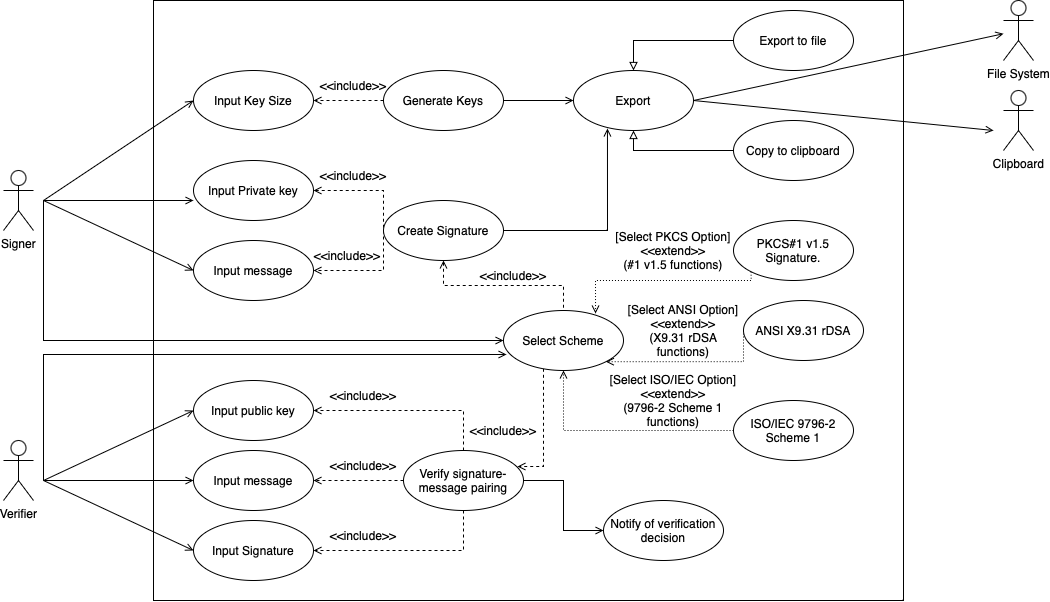
\includegraphics[scale=0.48]{POC_USE-CASE.png}
    \caption{UML Use Case Diagram}
    \label{fig:uc}
\end{figure}



\textbf{Generate Keys Use Case}

\noindent\textbf{Flow of Events:}
\begin{enumerate}
    \item User selects "Generate Key" from the main menu options panel.
    \item User is presented with an input box labeled "Input Key Size".
    \item User inputs desired key size into the box.
    \item System processes the request and generates the public-private key pair.
    \item System displays a notification informing the user that the key generation process was successful.
    \item User is presented with options "Export to file" and "Copy to clipboard".
    \item User selects desired option to either save the keys to a file or copy them to clipboard.
\end{enumerate}

\noindent\textbf{Alternative flows:}
\begin{enumerate}
    \item[3a.] User inputs an invalid key size.
    \begin{enumerate}
        \item[3a1.] System warns user about the invalid input and prompts them to enter a valid key size again.
    \end{enumerate}
    \item[5a.] System encounters an error during key generation.
    \begin{enumerate}
        \item[5a1.] System displays an error message and prompts the user to try again.
    \end{enumerate}
\end{enumerate}



\textbf{Create Signature Use Case}

\noindent\textbf{Flow of Events:}
\begin{enumerate}
    \item User selects "Sign message" from the main menu options panel.
    \item User is presented with text boxes labeled "Input Private Key" and "Input Message".
    \item User inputs their private key and the message they wish to sign.
    \item User selects the desired signature scheme from options like "PKCS\#1 v1.5 Signature", "ANSI X9.31 rDSA", etc.
    \item System processes the input and computes the digital signature.
    \item System displays a notification informing the signer that the signing process was successful.
    \item User is presented with options "Export to file" and "Copy to clipboard".
    \item User selects desired option to either save the keys to a file or copy them to clipboard.
\end{enumerate}

\noindent\textbf{Alternative flows:}
\begin{enumerate}
    \item[3a.] User inputs an invalid or mismatched private key.
    \begin{enumerate}
        \item[3a1.] System warns user about the invalid input and prompts them to enter a valid key.
    \end{enumerate}
    \item[5a.] System encounters an error during signature creation.
    \begin{enumerate}
        \item[5a1.] System displays an error message and prompts the user to try again.
    \end{enumerate}
\end{enumerate}

\textbf{Verify Signature Use Case}

\noindent\textbf{Flow of Events:}
\begin{enumerate}
    \item User selects "Verify Signature" from the main menu options panel.
    \item User is presented with options to input the message, its corresponding signature, and the public key.
    \item User provides all required inputs.
    \item System processes the information and verifies the authenticity of the signature.
    \item System displays a notification with the result, either confirming the authenticity or notifying of a mismatch.
\end{enumerate}

\noindent\textbf{Alternative flows:}
\begin{enumerate}
    \item[3a.] User inputs mismatched or incorrect information.
    \begin{enumerate}
        \item[3a1.] System warns user about the incorrect input and suggests rechecking the inputs.
    \end{enumerate}
    \item[4a.] System encounters an error during verification.
    \begin{enumerate}
        \item[4a1.] System displays an error message and prompts the user to try again.
    \end{enumerate}
\end{enumerate}

Acceptance Tests

\textbf{1. Key Pair Generation:}
\begin{enumerate}
\item Open the application and locate the key generation section.
\item Input a valid key size into the provided text box and submit.
\item If key size is invalid no key is issued and the user is informed to try again. 
\item Observe that no exceptions or errors are displayed during the key generation process.
\item If there are errors during key generation the user is informed to try again.
\item Confirm that a notification is presented to the user upon successful key generation.
\item Check if there is an option to save the generated key pair to a file and perform a successful save.
\end{enumerate}

\textbf{2. Digital Signature Generation:}
\begin{enumerate}
\item Locate the signature generation section in the application.
\item Input a test message into the provided text box.
\item Use the browse option to provide a valid private key file.
\item If empty message or invalid file is provided, the user is informed to try again. 
\item Ensure no errors or exceptions are displayed during the signing process.
\item Confirm that a notification is presented to the signer upon successful signature generation.
\item Check for options to either copy the signature to clipboard or save it to a file and verify both functionalities.
\end{enumerate}

\textbf{3. Digital Signature Verification:}
\begin{enumerate}
\item Locate the signature verification section in the application.
\item Use the text box or file browse option to input the original test message.
\item Use the browse option to provide the generated signature file.
\item If empty message or invalid file is provided, the user is informed to try again. 
\item Ensure no errors or exceptions are displayed during the verification process.
\item Confirm that a notification is presented to the verifier upon successful verification.
\end{enumerate}

\textbf{4. Signature and Verification with PKCS\#1 v1.5:}
\begin{enumerate}
\item Set the application to use the PKCS\#1 v1.5 Signature Scheme.
\item Sign a test message and verify its signature using the previous steps. Ensure both processes succeed.
\end{enumerate}

\textbf{5. Signature and Verification with ANSI X9.31 rDSA:}
\begin{enumerate}
\item Set the application to use the ANSI X9.31 rDSA Signature Scheme.
\item Sign a test message and verify its signature using the previous steps. Ensure both processes succeed.
\end{enumerate}

\textbf{6. Signature and Verification with ISO/IEC 9796-2:2010 Scheme 1:}
\begin{enumerate}
\item Set the application to use the ISO/IEC 9796-2:2010 Signature Scheme 1.
\item Sign a test message (both with partial and full recovery) and verify its signature using the previous steps. Ensure both processes succeed.
\end{enumerate}
\section{Appendix A.3 Design}
\begin{figure}[H]
    \centering
    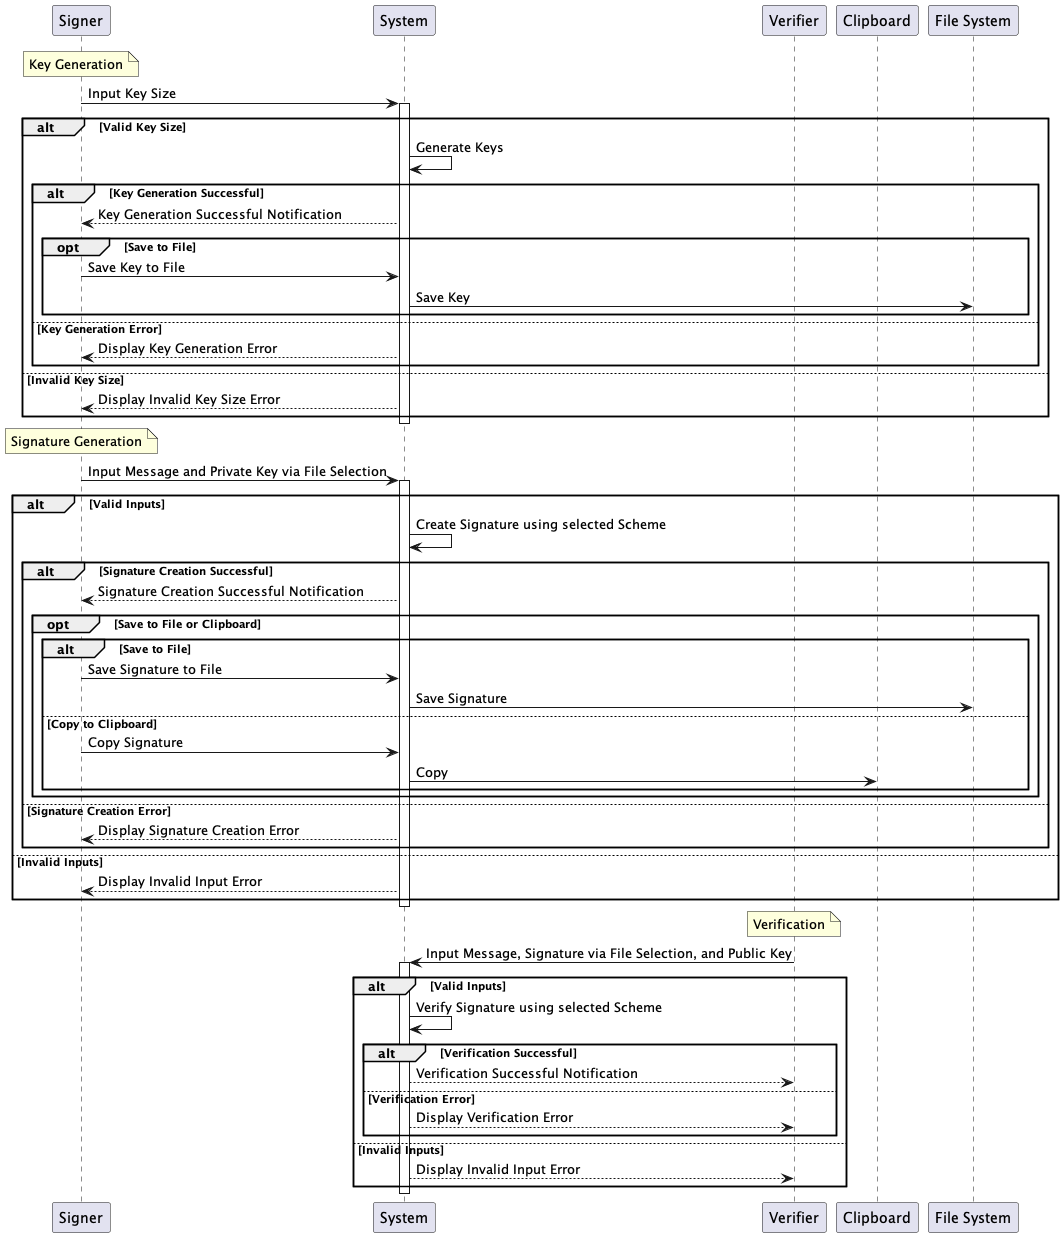
\includegraphics[scale=0.48]{sequence.png}
    \caption{UML Sequence Diagram}
    \label{fig:uc}
\end{figure}
Initially, the user is prompted to generate cryptographic keys, providing a key size that, if valid, leads to the creation of a private and public key pair. The user can then opt to save these keys onto their file system.

Once keys are in place, the user can sign a message. They input the message into the system and load their private key. If the inputs are correct, the system employs a chosen signature algorithm to create a digital signature, which the user can save or copy to their clipboard. In case of invalid input or an error during signature creation, the user is informed with an error message.

For verification, the user inputs a message, loads the digital signature and the corresponding public key. The system checks the signature against the message using the public key. If the signature is valid, a success notification is displayed; otherwise, the user is alerted to a verification error. Throughout this process, the system guides the user with notifications or error messages based on the success or failure of the operations performed.


%%%% ADD YOUR BIBLIOGRAPHY HERE
\newpage

\addcontentsline{toc}{chapter}{Bibliography}
\printbibliography
\label{endpage}
\end{document}

\end{article}
